\chapter{Working title}
\label{sec:something}


In the introduction to this project, we briefly discussed the scope and focus of the thesis. In figure/table .. we have displayed the complete list of structures, compositions and permutations of high-entropy silicides trialed throughout the duration of the project. \textbf{Make figure.} Amidst the large number of structures, we found particularly promising attributes of $(CrFeMnNi)Si_2$ (CFMN) SQSs based on the orthorombic crystal structure of $FeSi_2$, thus we will begin this section by presenting the results regarding this structure.

In this structure, each supercell consist of 48 total atoms, 32 of which is silicon, and the remaining 16 positions is equally distributed between Chromium, iron, manganese, and Nickel. The 5 distinct SQS supercells can be seen in figure (method/SQS). In table \ref{tab:FeSi2/CrFeMnNi_equal} we present a summary of the most relevant functional properties of the SQSs.

\begin{table}[H]
\centering
\begin{tabular}{@{}cccc@{}}
\toprule
Structure  & Total energy/atom (eV) & Final magnetic moment (?) & Band gap (eV) \\ \midrule
\textbf{A} & −6,6080                & 4.0006                    & 0.0280        \\
\textbf{B} & −6,6138                & 3.9999                    & 0.0523        \\
\textbf{C} & −6,6063                & 4.0008                    & 0.0344        \\
\textbf{D} & −6,6155                & 4.0001                    & 0             \\
\textbf{E} & −6,6089                & 4.0000                    & 0.0495        \\ \bottomrule
\end{tabular}
\caption{Total energy per atom, final magnetic moment, and band gap (GGA) of 5 $Cr_4Fe_4Mn_4Ni_4Si_{32}$ SQSs based on $FeSi_2$}
\label{table:fesi2_summary}
\end{table}  

Bellow we have plotted the total density of states corresponding to the five distinct SQSs.


\begin{table}[H]
\begin{tabular}{@{}ccc@{}}
\toprule
Structure  & Gap (D/I) & Transition                              \\ \midrule
\textbf{A} & I         & (0.500,0.333,0.500)-(0.500,0.000,0.000)  \\
\textbf{B} & I         & (0.250,0.000,0.250)-(0.000,0.000,0.000)  \\
\textbf{C} & -         & (0.500,0.000,0.500)-(-0.250,0.333,0.500) \\
\textbf{D} & I         & -                                        \\
\textbf{E} & I         & (0.000,0.000,0.000)-(0.250,0.000,0.250)  \\ \bottomrule
\end{tabular}
\caption{Band gap transition of CFMN (fesi2) SQSs with PBE functional}
\end{table}


\begin{figure}[H]
%\centering
\begin{subfigure}{0.5\textwidth}
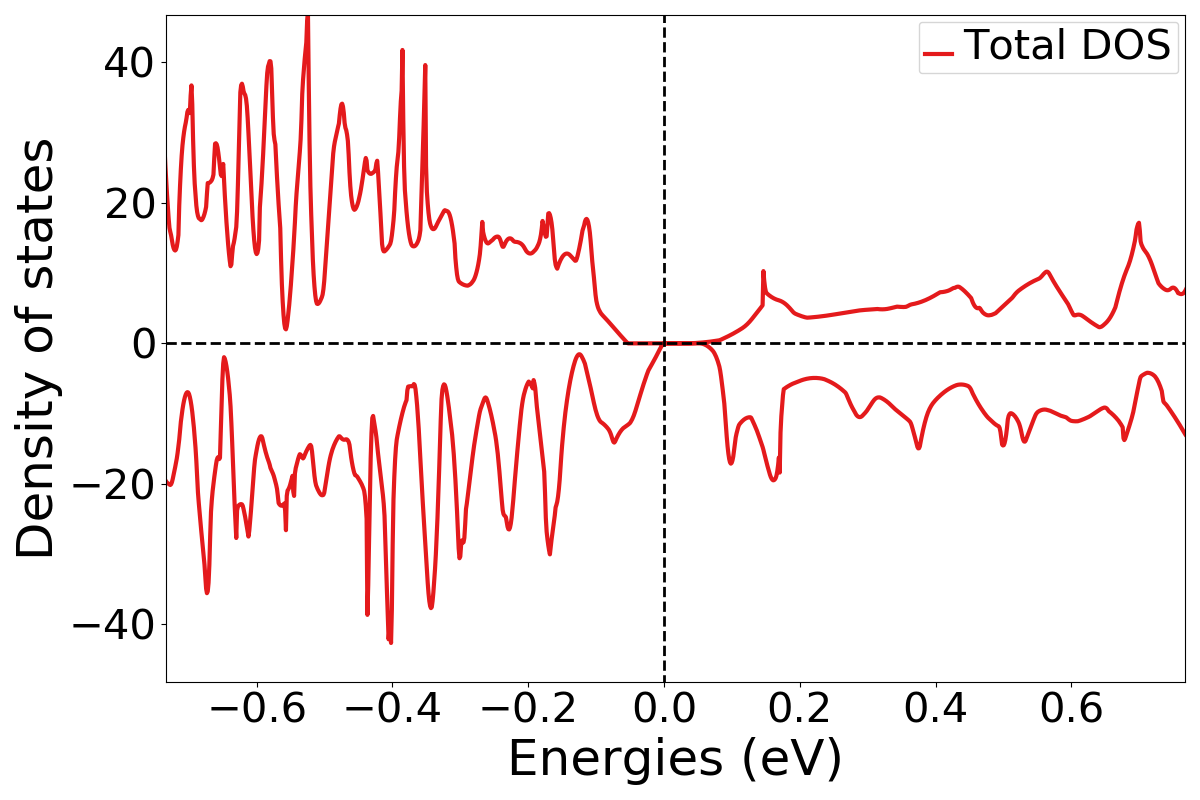
\includegraphics[width=\textwidth]{results/fesi2/DOS_A_toten.png}
\end{subfigure}
\begin{subfigure}{0.5\textwidth}
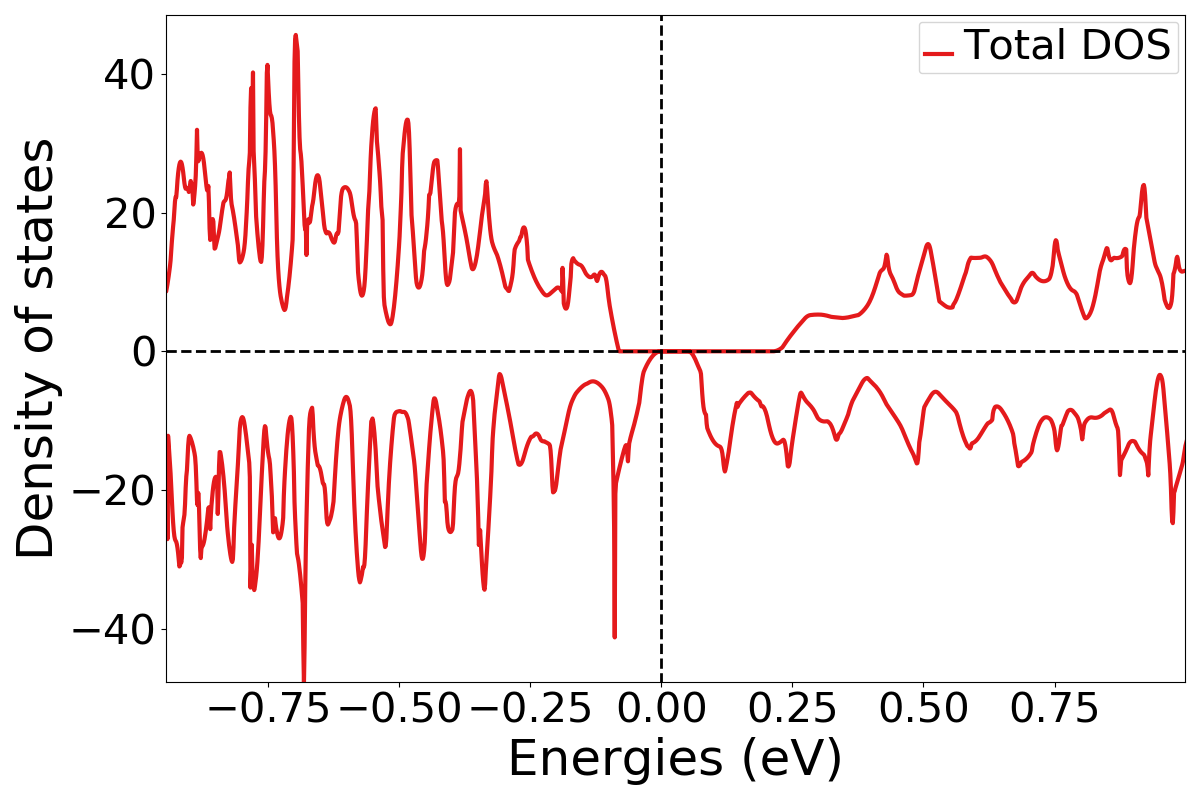
\includegraphics[width=\textwidth]{results/fesi2/DOS_B_toten.png}
\end{subfigure}
\begin{subfigure}{0.5\textwidth}
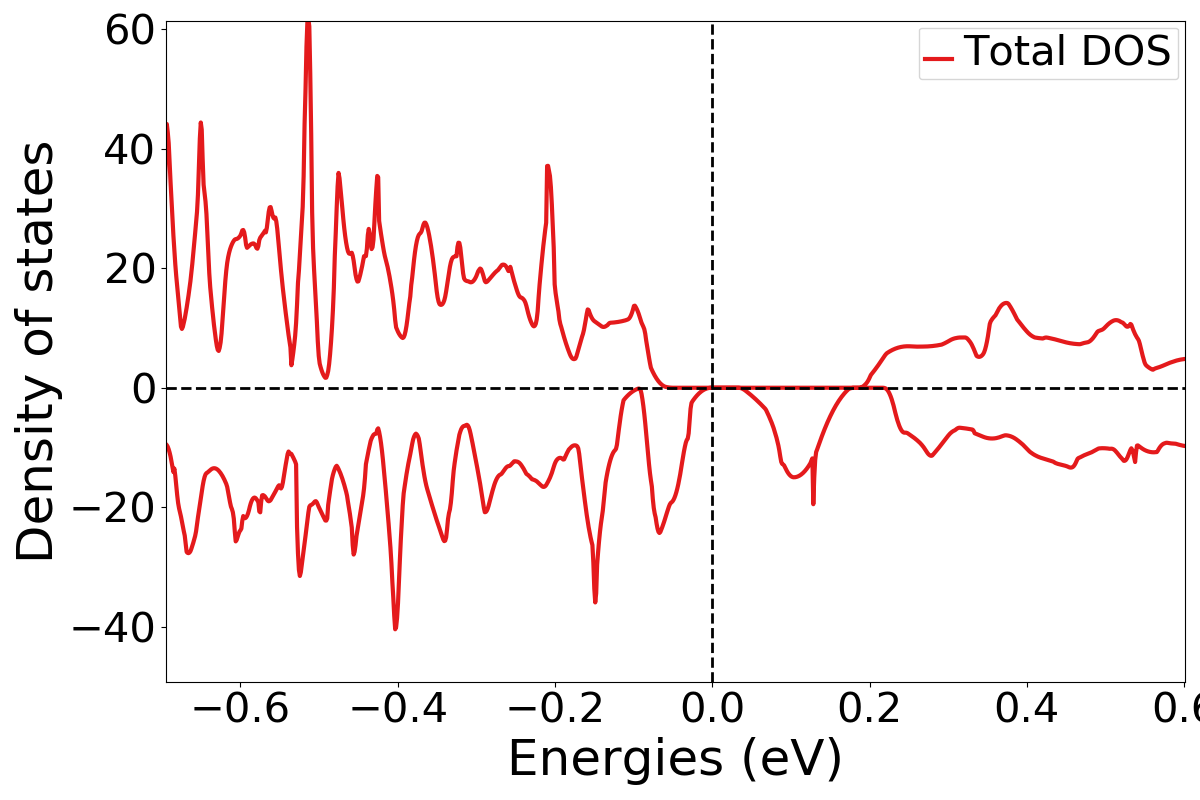
\includegraphics[width=\textwidth]{results/fesi2/DOS_C_toten.png}
\end{subfigure}
\begin{subfigure}{0.5\textwidth}
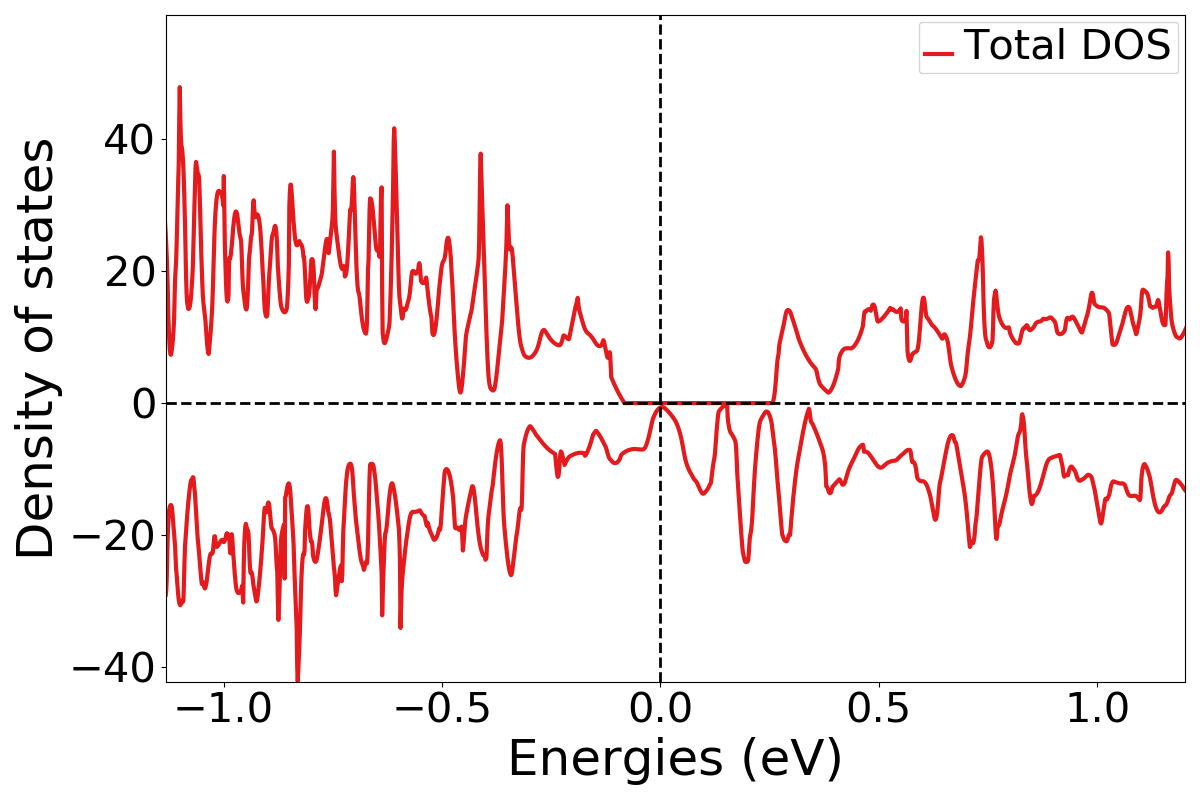
\includegraphics[width=\textwidth]{results/fesi2/DOS_D_toten.png}
\end{subfigure}
\begin{subfigure}{0.5\textwidth}
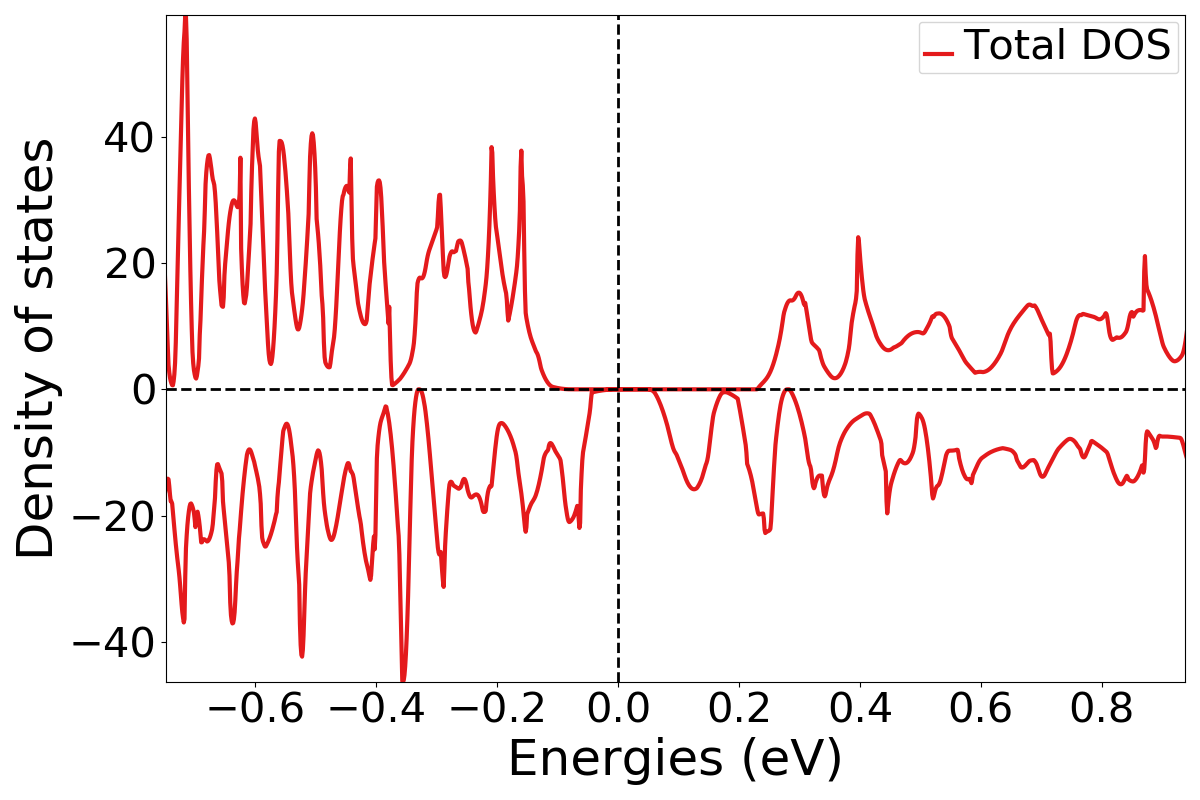
\includegraphics[width=\textwidth]{results/fesi2/DOS_E_toten.png}
\end{subfigure}
\caption{Density of states for structure A, B, C, D, E of $CFMNSi_2 (FeSi_2)$ SQSs (PBE GGA)}
\label{dos_fesi2_gga}
\end{figure}



\begin{comment}
\begin{table}[H]
\centering
\begin{tabular}{@{}cccc@{}}
\toprule
Structure  & Spin-up & Spin-down & Total  \\ \midrule
\textbf{A} & 0.0814  & 0.0522    & 0.0281 \\
\textbf{B} & 0.2932  & 0.0523    & 0.0523 \\
\textbf{C} & 0.2355  & 0.0343    & 0.0343 \\
\textbf{D} & 0.3386  & 0         & 0      \\
\textbf{E} & 0.3078  & 0.0495    & 0.0495 \\ \bottomrule
\end{tabular}
\caption{Band gap (GGA) in spin up and spin down channels of CFMNSi2 structures}
\end{table}

\begin{table}[H]
\centering
\begin{tabular}{@{}cccc@{}}
\toprule
Structure  & PBE    & SCAN   & HSE06  \\ \midrule
\textbf{A} & 0.0281 & 0.0000 & 0.0207 \\
\textbf{B} & 0.0523 & 0.0890 & 0.1808 \\
\textbf{C} & 0.0344 & 0.0690 & 0.0196 \\
\textbf{D} & 0.0000 & 0.0000 & 0.0000 \\
\textbf{E} & 0.0495 & 0.1048 & 0.0133 \\ \bottomrule
\end{tabular}
\caption{Band gap of $CFMN (FeSi_2)$ SQSs with GGA (PBE), meta-GGA (SCAN) and hybrid-functionals (HSE06). \textbf{Add footnote to explain the uncertainty in these results regarding smearing type and width, and DOS and EIGENVAL}}
\end{table}
\end{comment}


\begin{figure}[H]
\centering
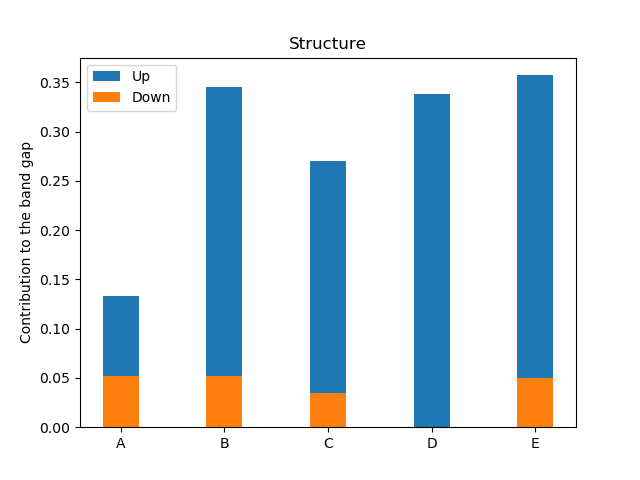
\includegraphics[scale=.7]{results/fesi2/spin_gap.png}
\caption{Band gap of CFMN fesi2 SQSs in spin up and spin down with PBE functional.}
\label{DOS_hse06_B}
\end{figure}

\begin{figure}[H]
\centering
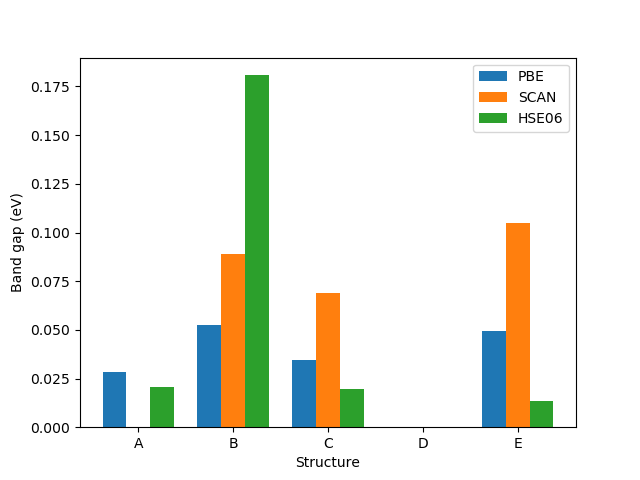
\includegraphics[scale=.7]{results/fesi2/xc_gap.png}
\caption{Band gap of CFMN (fesi2) all 5 SQSs with PBE, SCAN and HSE06}
\label{Xc_fig}
\end{figure}


Looking at the results from different functionals, we observe that the hybrid functional HSE06 more or less agree with results of the PBE functional in terms of the actual presence of the band gap, while the size of the gap is up for debate. Especially in B, where we observe a band gap greater than 0.18 eV in comparison to 0.05 eV with PBE and 0.08 with SCAN. Bellow we show the total density of states around the fermi energi $E_f$ for this structure with the HSE06 functional. 

\begin{figure}[H]
\centering
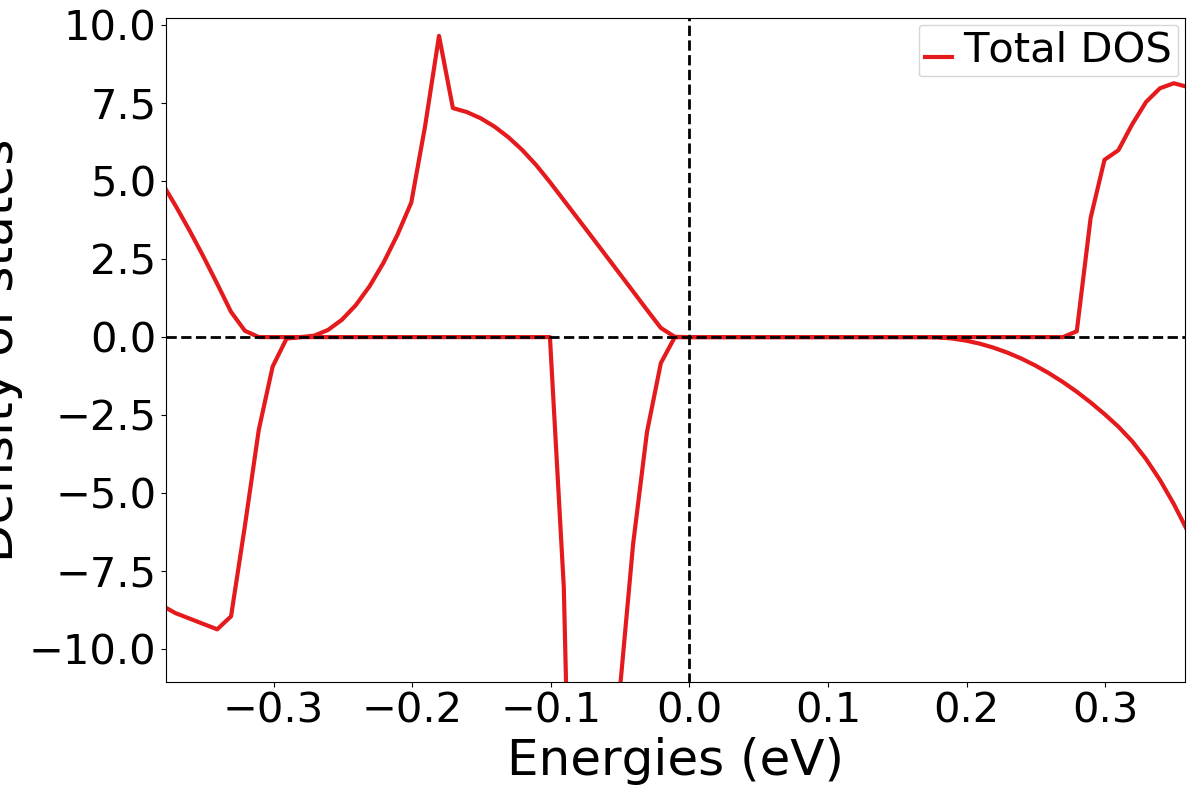
\includegraphics[scale=.3]{results/fesi2/hse06/B_DOS_zoom.png}
\caption{Density of states from HSE06 of $FeSi_2$ CFMN structure B}
\label{DOS_hse06_B}
\end{figure}

If we now compare this to the density of states of structure E,

\begin{figure}[H]
%\centering
\begin{subfigure}{0.5\textwidth}
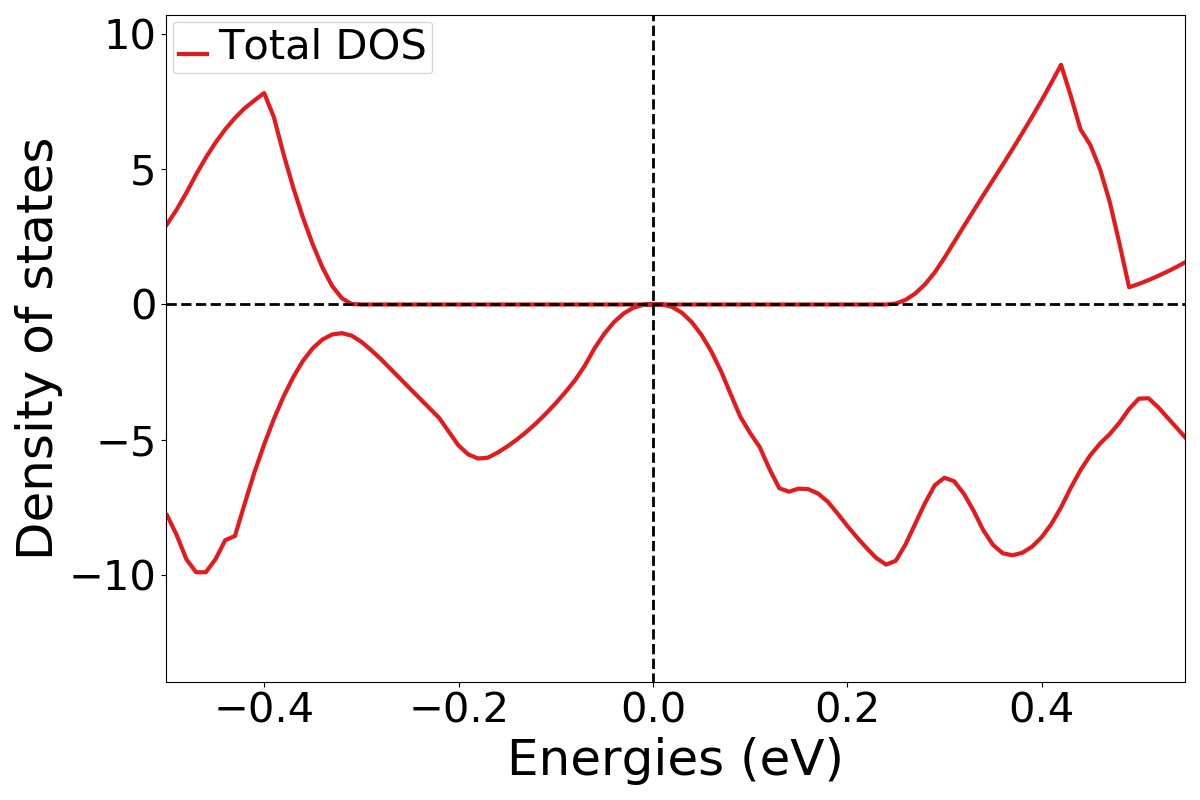
\includegraphics[width=\textwidth]{results/fesi2/hse06/E_DOS_zoom.png}
\caption{DOS $\uparrow, \downarrow$}
\end{subfigure}
\hfill
\begin{subfigure}{0.5\textwidth}
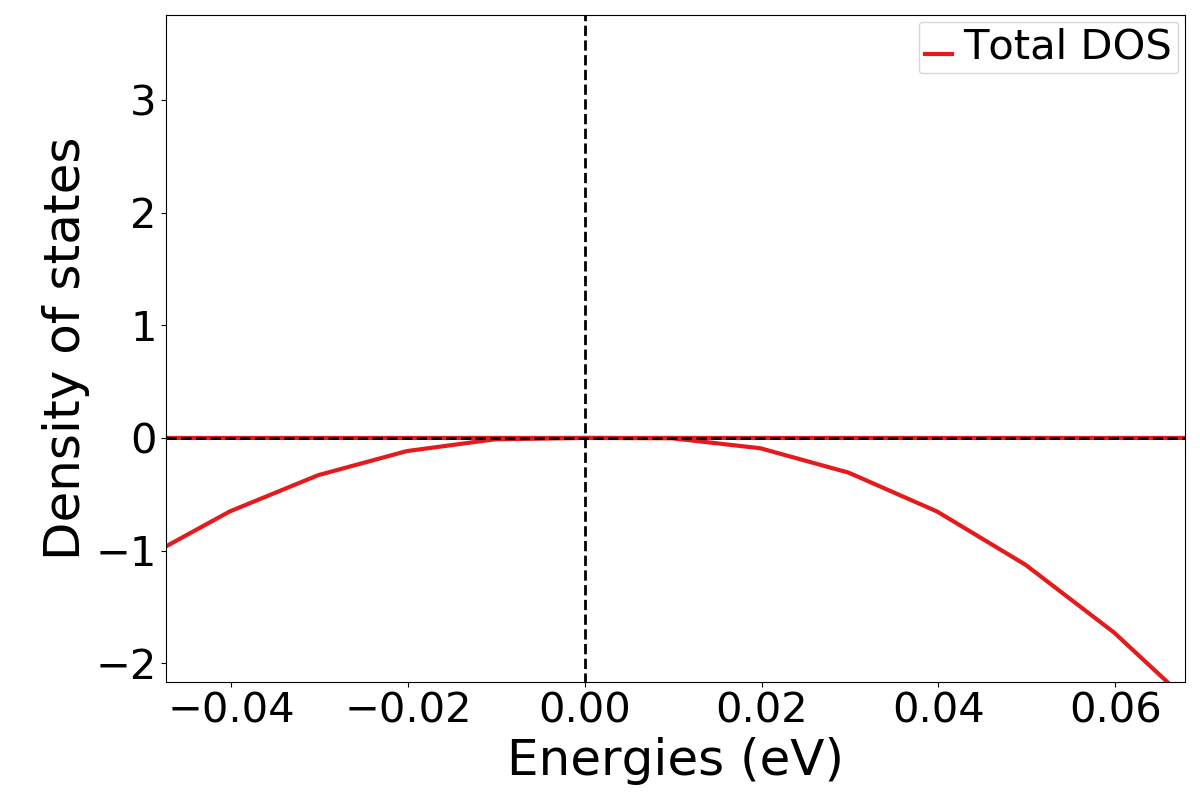
\includegraphics[width=\textwidth]{results/fesi2/hse06/E_DOS_down.png}
\caption{DOS $\downarrow$}
\end{subfigure}
\caption{The density of states of CFMN ($FeSi_2$) structure E for a) spin up and down, and b) focused on spin down}
\end{figure}

it's obvious that the wider band gap of structure B stems from the spin down channel, as opposed to the other structure where we observe large gaps in $\uparrow$ and small nonzero gaps in $\downarrow$ except for D with metallic characteristic in spin $\downarrow$, responsible for the zero band gap displayed in table ..

Now we will consider the local density of states of CFMN (fesi2). Bellow in fig .., we plot LDOS for all 5 structures \textbf{Fix figure placement and font later, need to add alpha to figure A like in the rest}
\newpage
\begin{figure}[H]
%\centering
	\begin{subfigure}{\textwidth}
		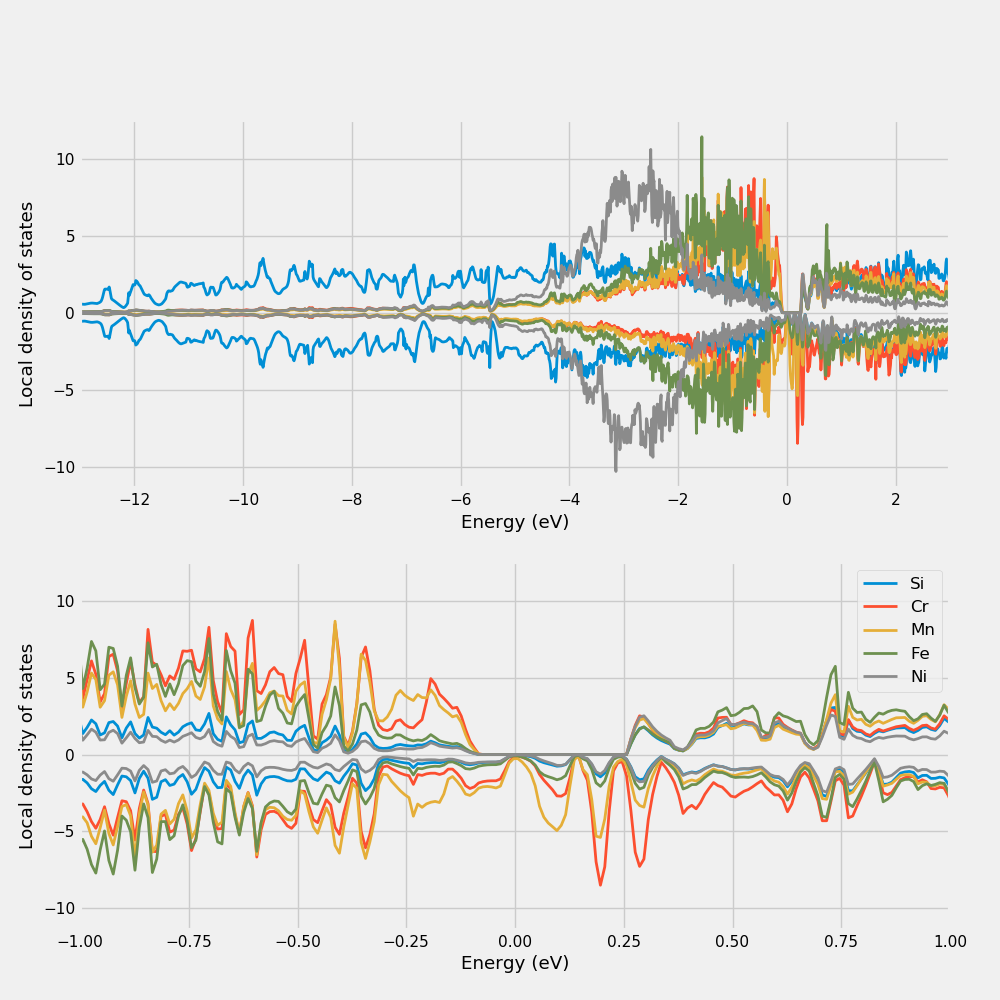
\includegraphics[width=\textwidth]{results/fesi2/A_LDOS.png}
		\caption{A}
	\end{subfigure}
	\begin{subfigure}{\textwidth}
		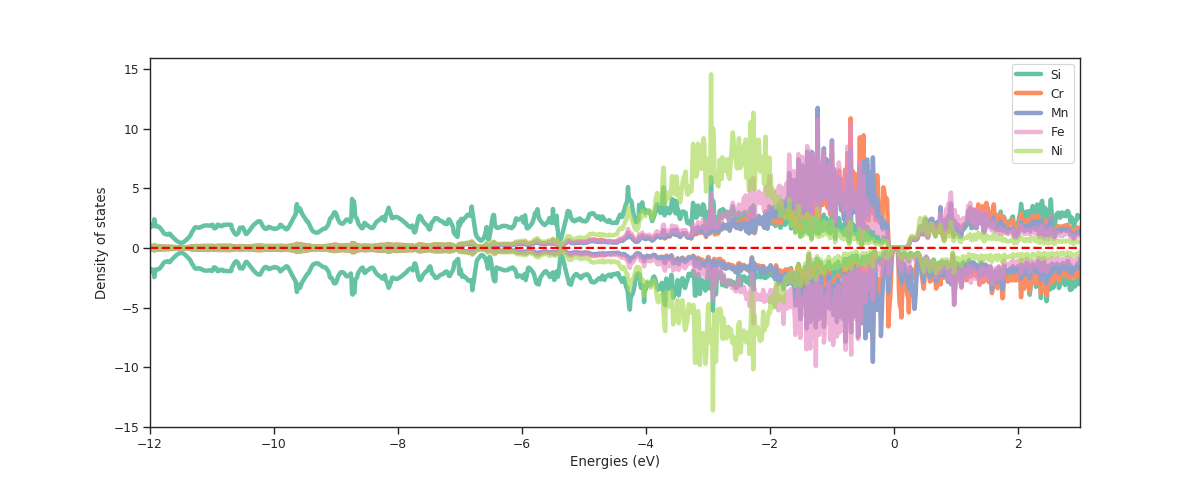
\includegraphics[width=\textwidth]{results/fesi2/B_LDOS.png}
		\caption{B}
	\end{subfigure}
	\begin{subfigure}{\textwidth}
		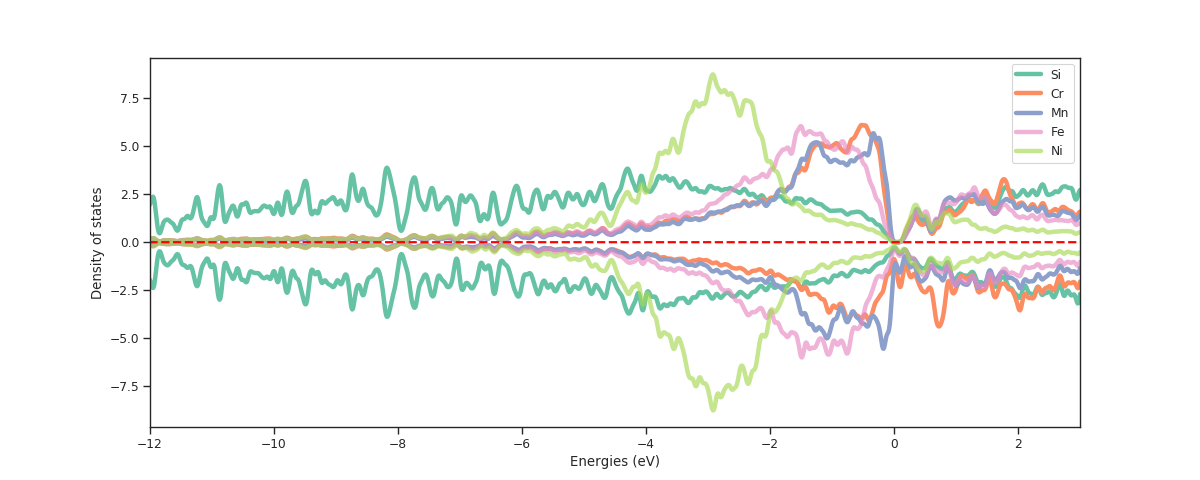
\includegraphics[width=\textwidth]{results/fesi2/C_LDOS.png}
		\caption{C}
	\end{subfigure}
	\begin{subfigure}{\textwidth}
		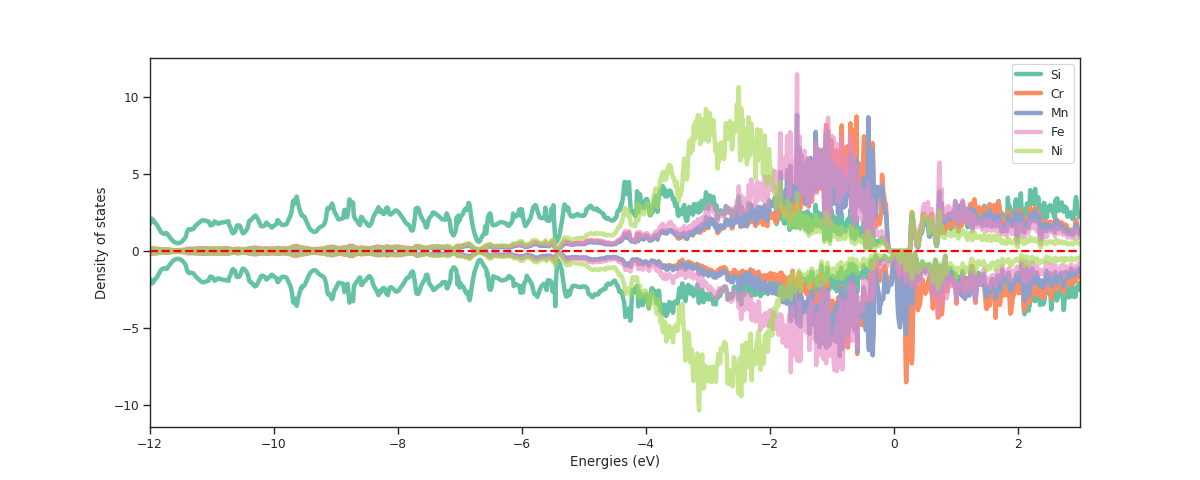
\includegraphics[width=\textwidth]{results/fesi2/D_LDOS.png}
		\caption{D}
	\end{subfigure}
\end{figure}		
\begin{figure}[H]
	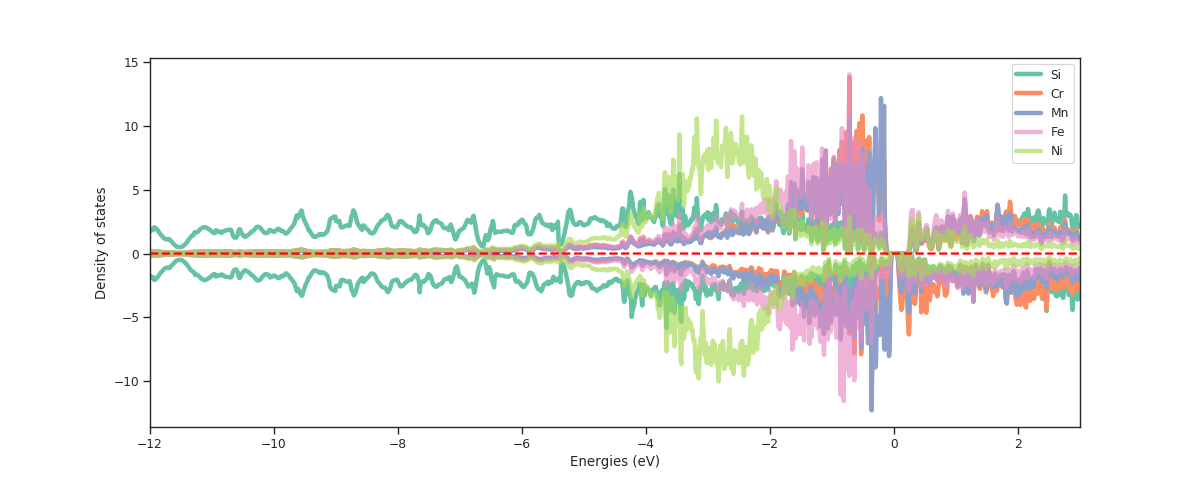
\includegraphics[width=\textwidth]{results/fesi2/E_LDOS.png}
	\caption{E}
\end{figure}

Next, we present the radial/probability distribution functions (R(P)DFs)

\begin{figure}[H]
%\centering
	\begin{subfigure}{\textwidth}
		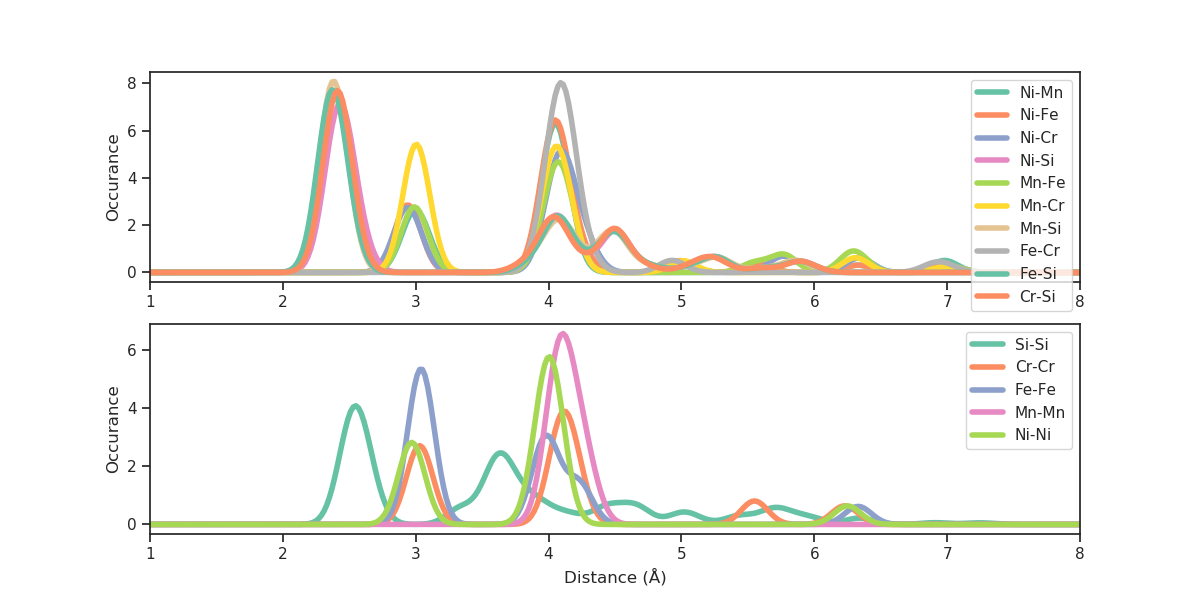
\includegraphics[width=\textwidth]{results/fesi2/A_PDF.png}
		\subcaption{A}
	\end{subfigure}	
	\begin{subfigure}{\textwidth}
		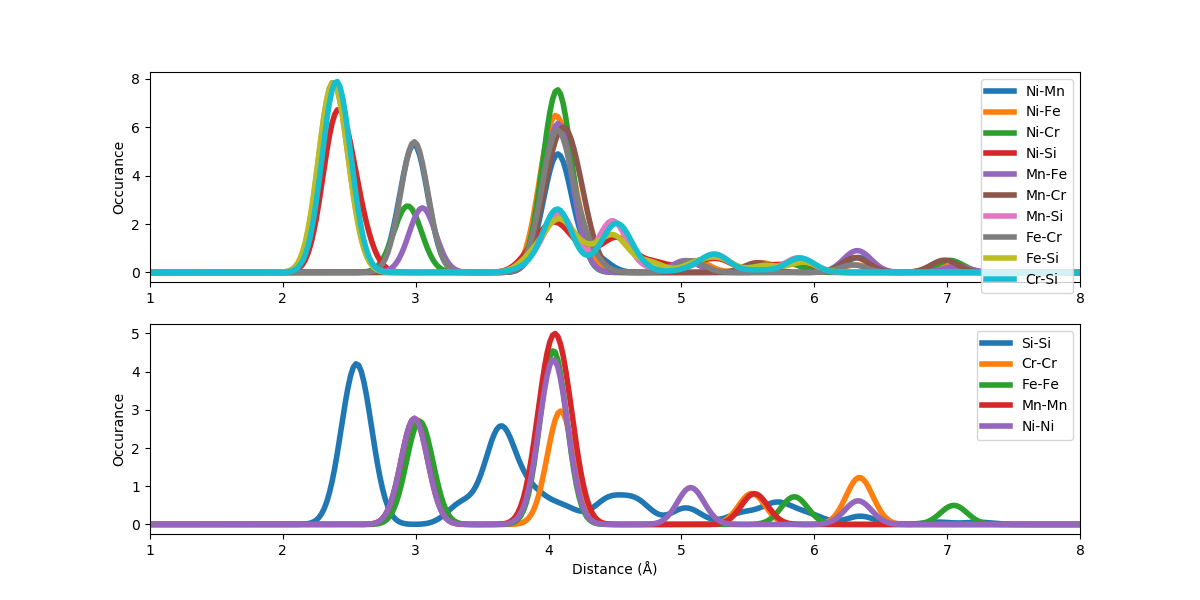
\includegraphics[width=\textwidth]{results/fesi2/B_PDF.png}
		\subcaption{B}
	\end{subfigure}
	\begin{subfigure}{\textwidth}
		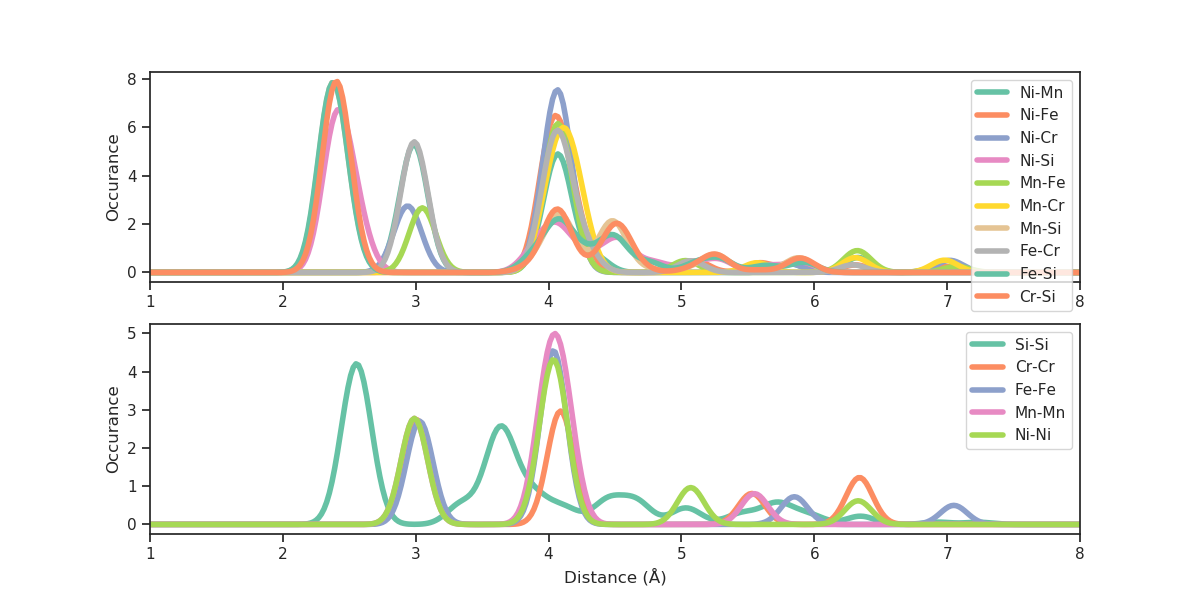
\includegraphics[width=\textwidth]{results/fesi2/C_PDF.png}
		\subcaption{C}
	\end{subfigure}
\end{figure}
\begin{figure}[H]
	\begin{subfigure}{\textwidth}
		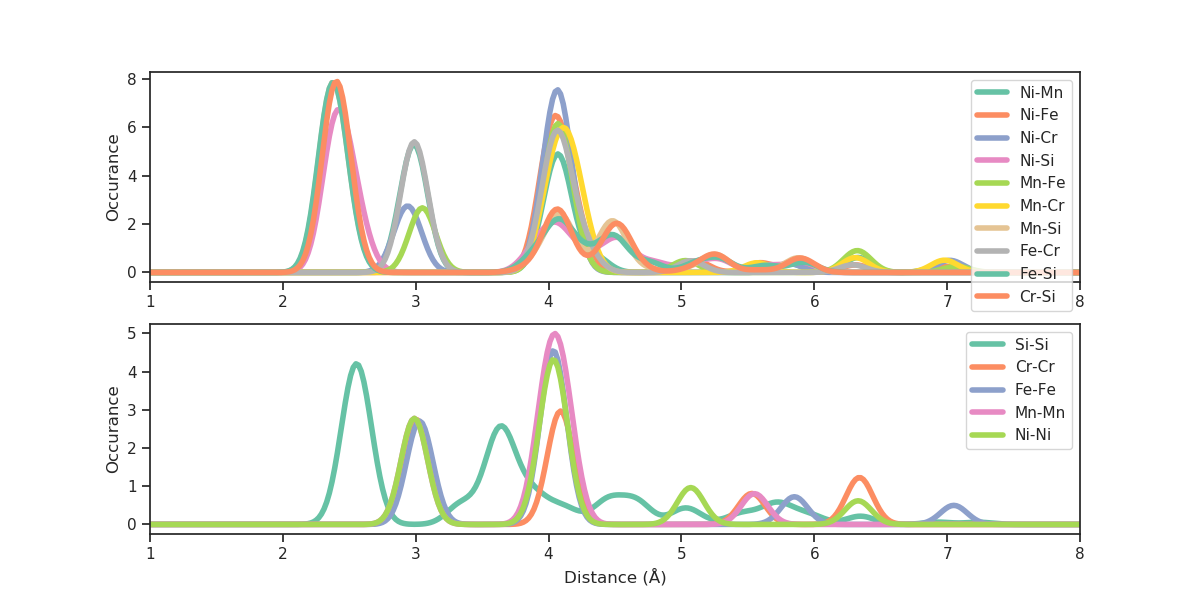
\includegraphics[width=\textwidth]{results/fesi2/D_PDF.png}
		\subcaption{D}
	\end{subfigure}
	\begin{subfigure}{\textwidth}
		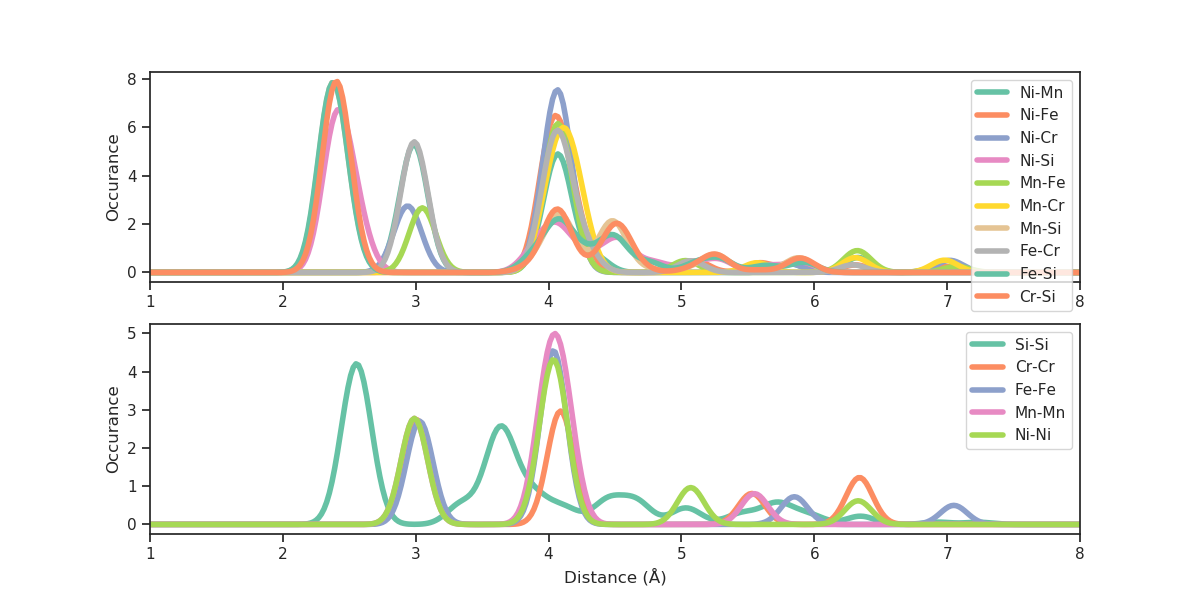
\includegraphics[width=\textwidth]{results/fesi2/E_PDF.png}
		\subcaption{E}
	\end{subfigure}
\end{figure}

And in final the charge density 

\begin{figure}
	\begin{subfigure}{0.5\textwidth}
		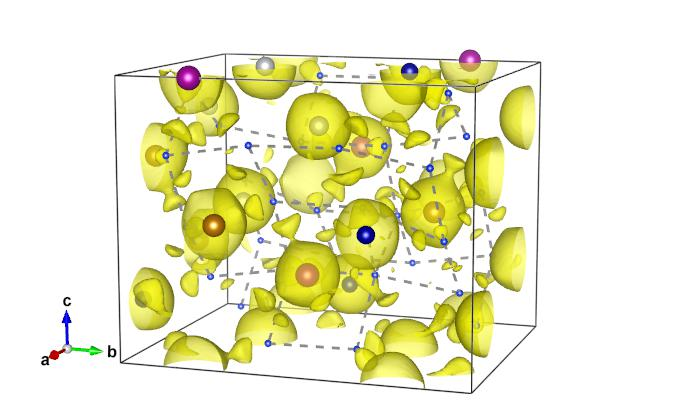
\includegraphics[width=\textwidth]{results/fesi2/A_CHGCAR.jpg}
		\caption{Structure A}
	\end{subfigure}
	\hfill
	\begin{subfigure}{0.5\textwidth}
		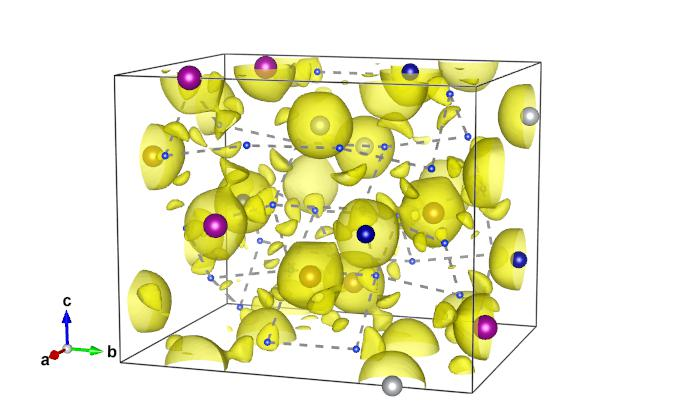
\includegraphics[width=\textwidth]{results/fesi2/B_CHGCAR.jpg}
		\caption{Structure B}
	\end{subfigure}
	\begin{subfigure}{0.5\textwidth}
		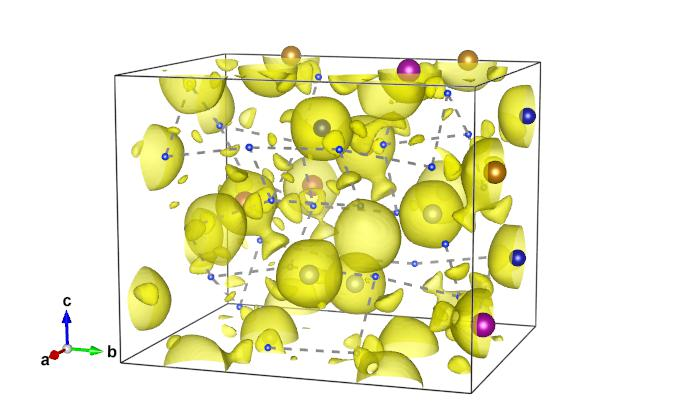
\includegraphics[width=\textwidth]{results/fesi2/C_CHGCAR.jpg}
		\caption{Structure C}
	\end{subfigure}
	\hfill
	\begin{subfigure}{0.5\textwidth}
		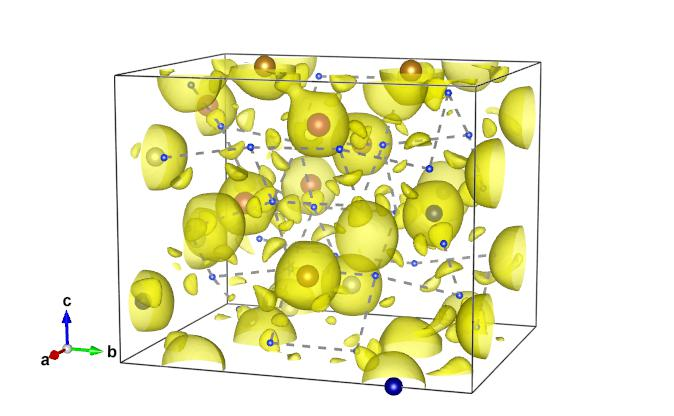
\includegraphics[width=\textwidth]{results/fesi2/D_CHGCAR.jpg}
		\caption{Structure D}
	\end{subfigure}
	\begin{subfigure}{0.5\textwidth}
		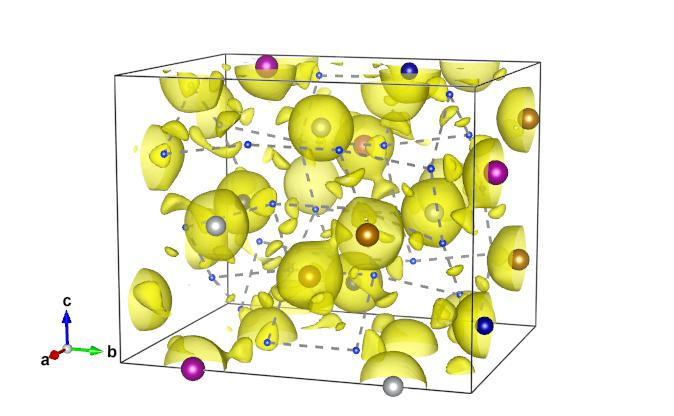
\includegraphics[width=\textwidth]{results/fesi2/E_CHGCAR.jpg}
		\caption{Structure E}
	\end{subfigure}
		\caption{Charge density}
		\label{chgcar}
\end{figure}


\textbf{I think its relevant and interesting to in-depth analyze structure B, D, and E. B because of large band gap. D because no band gap, and E because this well represents the other structures A and C. }
One difference is the KS eigenvalues. Str D have both partial occupancy and nonphysical occupancy, ie above 1 and bellow zero both in PBE and HSE06. This is not the case for structures that exhibited band gaps. Here we have clear transition from 1 to 0. Without having done a broad investigation of all material. This seems to be the case in other compositions and cells and permutations as well. Where both partial occupants and nonphysical occupations result in metallic structures. Calculating the band gap with strict 1 and 0 conditions, lead to small band gaps in most structures. Furthermore, in structures of Fe2Si, the difference in band where occupation transition from 1 to 0 between up and down, increases hugely compared to FeSi2 structures, talking close to 20 bands, opposed to maybe 2-5. 
